\title{Homework 2: ML Pipeline}

\author{Jean Salac (salac@uchicago.edu)}

\documentclass[letterpaper,12pt]{article}
\usepackage[letterpaper, portrait, margin = 0.5 in]{geometry}
\usepackage{graphicx}
\graphicspath{{images/}}
\usepackage{enumitem}
\usepackage{hyperref}

\begin{document}
\maketitle
\begin{center}
GitHub Repo: \url{https://github.com/jeansalac/ml-ppol} \\
Collaborator: Yuliana Zamora
\end{center}
\begin{enumerate}
\item \textbf{Read Data:} 
\begin{itemize}
\item To read in the csv file, I wrote a function in my library \textit{pipeLib.py} called  that takes in the csv file through command line and converts it to a data frame using the PANDAS library function \textit{read\_csv()}. 
\end{itemize}


\item \textbf{Explore Data:}
\begin{itemize}
\item \underline{\textit{dataSummary(dataFrame,var)}}: This function takes in a \textit{dataFrame} object and \textit{var}, the variable you would like a data summary for and returns the summary statistics of \textit{var}. Running this function on the variable \textit{age} in \textit{pipeTest.py} yields:
\begin{center}
\begin{tabular}{c c}
count  &  41016.000000 \\
mean   &     51.683489 \\
std    &     14.746880 \\
min    &     21.000000 \\
$25\%$    &     41.000000 \\
$50\%$    &     51.000000 \\
$75\%$    &     62.000000 \\
max    &    109.000000 \\
\end{tabular}
\end{center}

\newpage

\item \underline{\textit{varDist(dataFrame,var)}}: This function takes in a \textit{dataFrame} object and $var$, the variable you would like to see a distribution plot for and returns a distribution plot of $var$. Running this function on variable \textit{numberOfDependents} results in the plot below:
\begin{center}
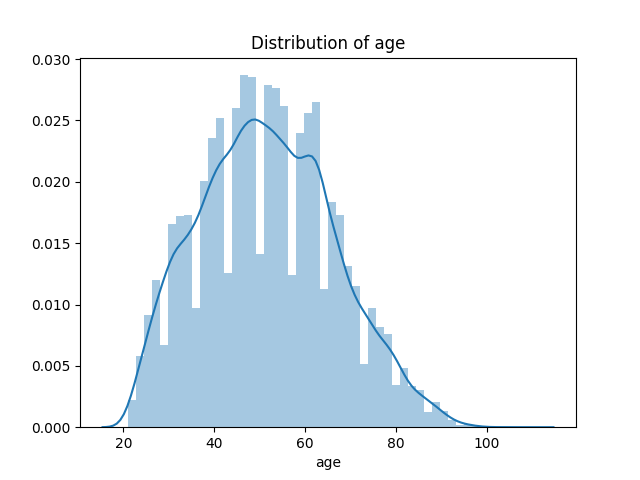
\includegraphics[scale=.5]{varDist.png}
\end{center}

\item \underline{\textit{corrSummary(dataFrame)}}: This function takes in a \textit{dataFrame} and returns a heatmap of the correlations between all the variables. Running this on the credit data results in the heatmap below.
\begin{center}
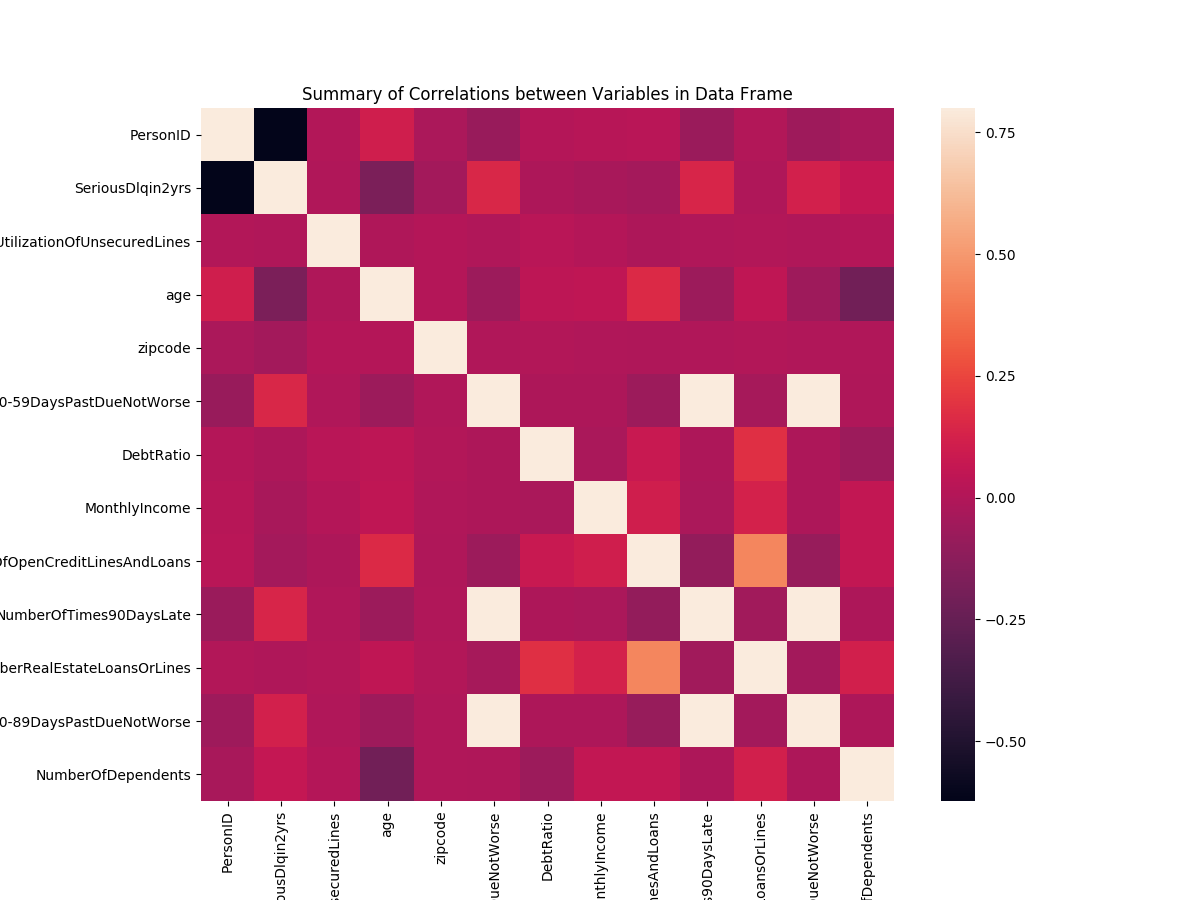
\includegraphics[scale=.6]{corrSummary.png}
\end{center}

\newpage

\item \underline{\textit{plotCorr(dataFrame,list)}}: This function takes in a \textit{dataFrame} object and a list of variables you would like to see a correlation for. It returns a plot of all the correlations for the variables provided. Running this on the variables \textit{RevolvingUtilizationOfUnsecuredLines, NumberOfOpenCredit-LinesAndLoans, NumberRealEstateLoansOrLines} results in the plot below: \\
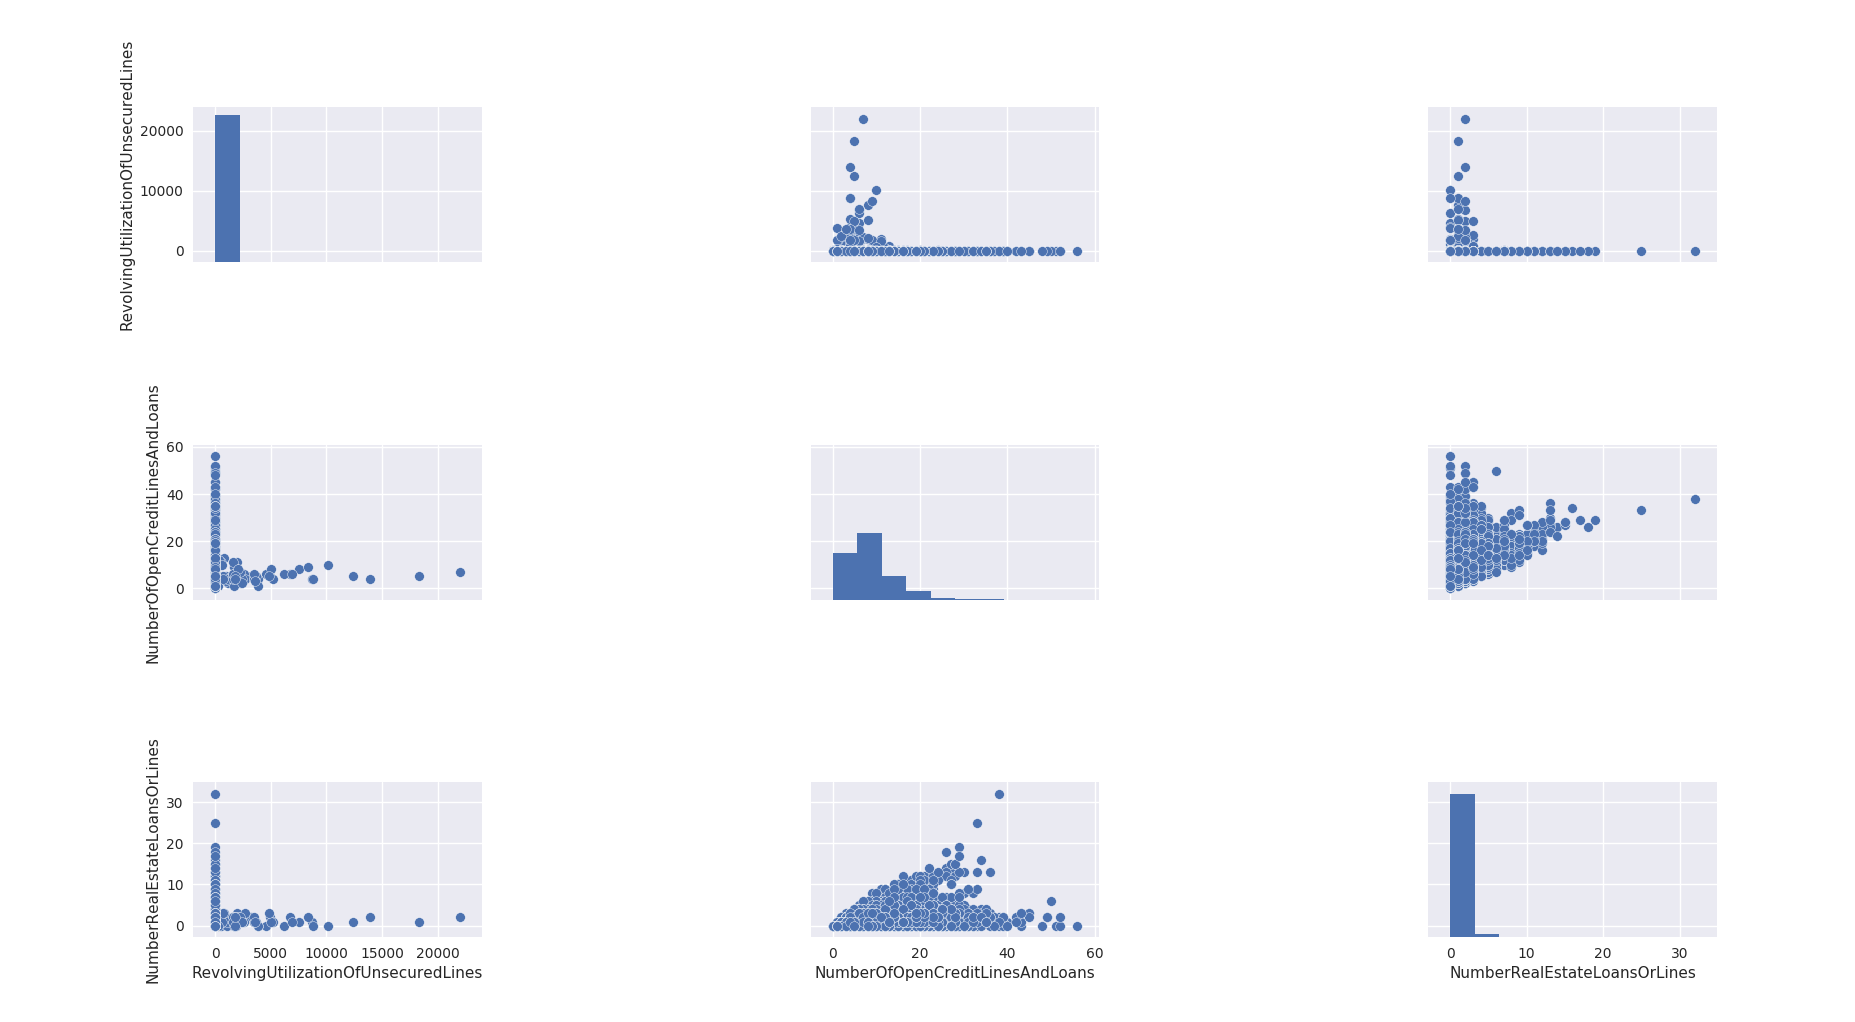
\includegraphics[scale=0.4]{plotCorr.png}


\item \underline{\textit{findLowOutliers(dataFrame,var, num)}}: This function takes in a \textit{dataFrame} object, the variable \textit{var} you want to find low outliers for, and the number of outliers you want \textit{num}. Running this function on \textit{debtRatio} to find the 3 lowest outliers yields the following array: \\ $[-0.25573621, -0.25573621,-0.25573621]$


\item \underline{\textit{findHighOutliers(dataFrame,var,num)}}: This function takes in a \textit{dataFrame} object, the variable \textit{var} you want to find high outliers for, and the number of outliers you want \textit{num}. Running this function on \textit{debtRatio} to find the 10 highest outliers yields the following array: \\ $[18.64412907,18.71742623,20.32533443,23.11834196,25.08424891,$ \\
$29.6749657, 30.88552614, 37.63658024,46.20077458,82.21128292]]$

\newpage

\item \underline{\textit{findBivariateOutliers(dataFrame,varX, varY,maxY)}}: This function takes in a \textit{dataFrame} object, the variable \textit{varX} you want to be plotted on the x-axis,\textit{varY} you want to be plotted on the y-axis, and \textit{maxY}, the upper limit of \textit{varY}. Running this function \textit{age} and \textit{numberOfDependents} results in the plot below: \\
\begin{center}
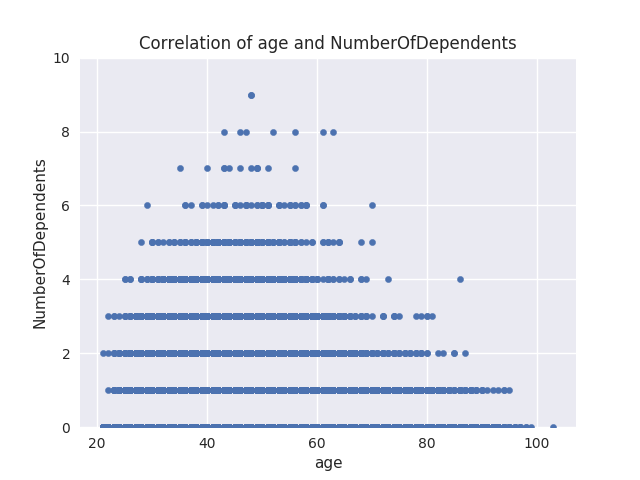
\includegraphics[scale=.7]{bivariateOutliers.png}
\end{center}
\end{itemize}


\item \textbf{Pre-Process Data:}
\begin{itemize}
\item \underline{\textit{fillMissing(dataFrame,var,newVal)}}: This function takes in the variable you want to fill in with missing data \textit{var} and the value you want the missing data to have \textit{newVal}. In $pipeTest.py$, I filled in the missing data for my continuous variables with that variable's median, and for the categorical variable \textit{zipcode}, I filled missing values with $0$.
\end{itemize}


\item \textbf{Generate Features and Predictors:}
\begin{itemize}
\item \underline{\textit{discretize(dataFrame,var,num)}}: This function takes in the variable \textit{var} you want to discretize and \textit{num}, the number of bins you want to discretize \textit{var} into. Running this function discretizes \textit{age} into the following 5 bins: 
\begin{enumerate}
\item (20.912, 38.6]
\item (38.6, 56.2] 
\item (56.2, 73.8] 
\item (73.8, 91.4]
\item (91.4, 109.0]
\end{enumerate}
\item \underline{\textit{createDummy(dataFrame,var)}}: This function takes in the variable \textit{var} you want to create dummy variables for. Running this function generates the following dummy variables for \textit{zipcode} $[60601,60618,60625,60629,60637,60644]$
\end{itemize}

\newpage

\item \textbf{Build Classifier:}
\begin{itemize}
\item \underline{\textit{logReg(dataFrame,IV,listOfDVs)}}: This function takes in the independent variable \textit{IV} and the dependent variables \textit{listOfDVs} you want to generate a logistic regression for. It returns the coefficients of the logistic regression, as well as its accuracy with the original data. Running this on the credit data resulted in $83.4\%$ accuracy with the original data, as well as the following coefficients: \\
\begin{tabular}{c c}
Intercept & [1.7464243465145182e-06]\\
RevolvingUtilizationOfUnsecuredLines & [-0.00016337547191778968] \\
age & [-0.03262736739776818] \\
zipcode & [5.897286708290562e-07] \\
NumberOfTime30-59DaysPastDueNotWorse & [0.04751821911375464] \\
DebtRatio & [-7.298373065337037e-05] \\
MonthlyIncome & [-3.17536592389569e-05] \\
NumberOfOpenCreditLinesAndLoans & [0.00987689310445205] \\
NumberOfTimes90DaysLate & [0.03450484254010904] \\
NumberRealEstateLoansOrLines & [0.006558732565761694] \\
NumberOfTime60-89DaysPastDueNotWorse") & [0.018844760061179952] \\
NumberOfDependents & [0.011227895523920409] \\
\end{tabular} \\
\end{itemize}


\item \textbf{Evaluate Classifier:} \\
If we evaluate this classifier on accuracy with the original data, then an $83.4\%$ accuracy is reasonably good. At the very least, it does better than random, which results in a $16.7\%$ accuracy. However, since we are only evaluating this model on the same data it trained on, this could be a case of overfitting. We do not know how this model will behave with new data points.
\end{enumerate}
\end{document}